\documentclass[oneside,14pt]{extarticle}
\usepackage[utf8]{inputenc}
\usepackage[english,ukrainian]{babel}
\usepackage{amssymb,amsfonts,amsmath,amsthm,mathtext,textcomp}

\usepackage[includehead, headsep=0pt, footskip=0pt, top=2cm, bottom=2cm, left=2cm, right=1cm]{geometry}
\usepackage{indentfirst}
\usepackage[onehalfspacing]{setspace}
\usepackage[headings]{fancyhdr}
\usepackage{etoolbox}
\usepackage{flafter}
\usepackage{listings}
\usepackage{graphicx}
\usepackage{float}
\usepackage[labelsep=period]{caption}

\usepackage{array}
\fancyhf{}
\renewcommand{\headrulewidth}{0pt}
\pagestyle{fancy}
\fancyfoot[R]{\thepage}
\lstset{breaklines=true,}
\graphicspath{ {./pictures} }

\lstset{
	language=c,
	tabsize=4,
	keepspaces,
	showstringspaces=false,
}
\graphicspath{ {./pictures} }
\setlength{\parindent}{4em}

\newcommand\subject{Моделювання та аналіз програмного забезпечення}
\newcommand\lecturer{доцент кафедри ПЗ \\ Сердюк П.В.}
\newcommand\teacher{викладач кафедри ПЗ \\ Микуляк А.В.}
\newcommand\mygroup{ПЗ-22}
\newcommand\lab{2}
\newcommand\theme{Класи, інтерфейси і структури у
	мові програмування С\#}
\newcommand\purpose{Ознайомлення з основами класів, структур, та інших базових
	елементів мови програмування С\#}

\begin{document}
\begin{normalsize}
	\begin{titlepage}
		\thispagestyle{empty}
		\begin{center}
			\textbf{МІНІСТЕРСТВО ОСВІТИ І НАУКИ УКРАЇНИ\\
				НАЦІОНАЛЬНИЙ УНІВЕРСИТЕТ "ЛЬВІВСЬКА ПОЛІТЕХНІКА"}
		\end{center}
		\begin{flushright}
			\textbf{ІКНІ}\\
			Кафедра \textbf{ПЗ}
		\end{flushright}
		\vspace{70pt}
		\begin{center}
			\textbf{ЗВІТ}\\
			\vspace{10pt}
			до лабораторної роботи № \lab\\
			\textbf{на тему}: “\textit{\theme}”\\
			\textbf{з дисципліни}: “\subject”
		\end{center}
		\vspace{50pt}
		\begin{flushright}
			
			\textbf{Лектор}:\\
			\lecturer\\
			\vspace{10pt}
			\textbf{Виконав}:\\
			
			студент групи \mygroup\\
			Коваленко Д.М.\\
			\vspace{10pt}
			\textbf{Прийняв}:\\
			
			\teacher\\
			
			\vspace{28pt}
			«\rule{1cm}{0.15mm}» \rule{1.5cm}{0.15mm} 2023 р.\\
			$\sum$ = \rule{1cm}{0.15mm}……………\\
			
		\end{flushright}
		\vspace{\fill}
		\begin{center}
			\textbf{Львів — 2023}
		\end{center}
	\end{titlepage}
		
	\begin{description}
		\item[Тема.] \theme.
		\item[Мета.] \purpose.
	\end{description}

	\section*{Завдання}
	\begin{enumerate}
		\item Реалізувати ланцюжок наслідування у якому б був звичайний клас,
		абстрактний клас та інтерфейс. Перелічіть відмінності та подібності у цих
		структурах у звіті у вигляді таблиці.
		
		\item Реалізувати різні модифікатори доступу. Продемонструвати доступ до цих модифікаторів там де він є, та їх відсутність там, де це заборонено
		(включити в звіт вирізки з скріншотів Intelisense з VisualStudio).
	\end{enumerate}

	\section*{Хід виконання}
	\subsection*{Частина 1}
	\subsection*{Завдання 1}	
	\begin{table}[H]
		\centering
		\begin{tabular}{ |c|c|c| }
			\hline
			& \textbf{Class} & \textbf{Abstract Class} \\ 
			\hline
			\textbf{Inheritance} & Single & Single \\ 
			\hline
			\textbf{Implementation} & Full & Partial \\ 
			\hline
			\textbf{Fields} & Yes & Yes \\ 
			\hline
			\textbf{Properties} & Yes & Yes \\ 
			\hline
			\textbf{Methods} & Yes & Yes \\ 
			\hline
			\textbf{Constructors} & Yes & Yes \\ 
			\hline
			\textbf{Access Modifiers} & Public, Private, Protected, Internal & Public, Protected, Internal \\ 
			\hline
			\textbf{Instantiation} & Can create objects & Cannot create objects \\ 
			\hline
		\end{tabular}
	\end{table}
	
	\begin{table}[H]
		\centering
		\begin{tabular}{ |c|c| }
			\hline
			& \textbf{Interface} \\ 
			\hline
			\textbf{Inheritance} & Multiple \\ 
			\hline
			\textbf{Implementation} & None \\ 
			\hline
			\textbf{Fields} & No \\ 
			\hline
			\textbf{Properties} & No \\ 
			\hline
			\textbf{Methods} & Yes \\ 
			\hline
			\textbf{Access Modifiers} & Public \\ 
			\hline
			\textbf{Instantiation} & Cannot create objects \\ 
			\hline
		\end{tabular}
		\caption{Відмінності та подібності класу, абстрактного класу та інтерфейсу.}
	\end{table}
	
	\subsection*{Завдання 2}
		\begin{figure}[H]
		\centering
		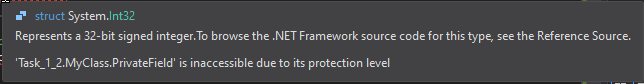
\includegraphics[scale=0.7]{1_2_1}
		\caption{Помилка використання private field.}
	\end{figure}
	
	\begin{figure}[H]
		\centering
		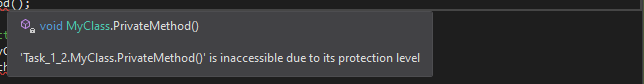
\includegraphics[scale=0.7]{1_2_2}
		\caption{Помилка використання private method.}
	\end{figure}
	
	\begin{figure}[H]
		\centering
		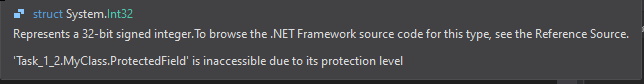
\includegraphics[scale=0.7]{1_2_3}
		\caption{Помилка використання protected field.}
	\end{figure}
	
	\begin{figure}[H]
		\centering
		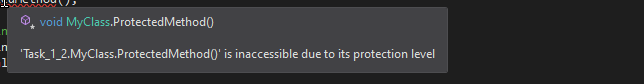
\includegraphics[scale=0.7]{1_2_4}
		\caption{Помилка використання protected method.}
	\end{figure}

	\subsection*{Завдання 3}
	Доступом за замовчуванням для всього в C\# є "найбільш обмежений доступ, який ви можете оголосити для цього члена".
	
		\begin{table}[H]
		\centering
		\begin{tabular}{ |c|c| }
			\hline
			\textbf{Member Type} & \textbf{Default Access Modifier} \\ 
			\hline
			namespace & public \\ 
			\hline
			enum & public \\ 
			\hline
			interface & internal \\ 
			\hline
			class & internal \\ 
			\hline
			struct & internal \\ 
			\hline
			delegate & internal \\ 
			\hline
		\end{tabular}
		\caption{Доступ за замовчуванням для не вкладених типів.}
	\end{table}
	
	\begin{table}[H]
		\centering
		\begin{tabular}{ |c|c| }
			\hline
			\textbf{Member Type} & \textbf{Default Access Modifier} \\ 
			\hline
			namespace & public \\
			\hline
			enum & public \\
			\hline
			interface & public \\
			\hline
			class & private \\
			\hline
			struct & private \\
			\hline
			delegate & private \\
			\hline
			constructor & private \\ 
			\hline
			enum member & public\\ 
			\hline
			interface member & public \\ 
			\hline
			method & private \\ 
			\hline
			field & private \\  
			\hline
			property & private \\  
			\hline
		\end{tabular}
		\caption{Доступ за замовчуванням для вкладених типів.}
	\end{table}
		
	\subsection*{Завдання 4}
	Модифікатор доступу до поля може бути встановленим не більшим ніж тип цього поля.
		
	\section*{Результати}

	\section*{Висновки}

	    
\end{normalsize}
\end{document}
